\part{Partie Theorique}
\chapter{Introduction Au systeme temps réel}
\minitoc
\section{Introduction}
\section{Taxonomie sur les systèmes temps réel}
\subsection*{Différents niveaux de criticité}
\vspace{-1cm}
Les systèmes temps réel dits critiques (ou dur) correspondent ont des systèmes pour lesquelles il est intolérable qu’une échéance soit manquée au risque de causer des conséquences graves, telles que des blessures ou des pertes humaines. Les centrales nucléaires ou le guidage de missiles représentent de tels systèmes à haute criticité. Dans le domaine de l’informatique embarqué, l’automobile et l’aéronautique regorgent de systèmes critiques à l’image des équipements déclencheurs d’airbags ou des logiciels de contrôle de vol de satellite. Il est crucial que les résultats soient disponibles au moment voulu et un résultat obtenu trop tard est inutilisable, à l’instar d’un système anti-missile qui recevrait la position d’un objet volant avec du retard.
\\ \indent Les systèmes temps réels mou sont des systèmes où on tolère les retards et ne requièrent pas un déterminisme temporel aussi fort que les systèmes temps réels dur.
Par exemple, un logiciel de diffusion de flux vidéo produit un certain nombre d’images dans un intervalle de temps régulier. Le fait de manquer une ou plusieurs échéances ne provoque pas l’arrêt du système multimédia. La qualité de la vidéo est dégradée mais le service peut continuer de fonctionner sans risque. Donc les systèmes temps réels mou  offre le  meilleur service possible (notion de best effort) et les retards dans l’obtention des résultats ne sont pas dramatiques.
\\ \indent A la frontière entre les systèmes temps réel dur et mou, les systèmes temps réel ferme tolèrent une certaine proportion d’échéances manquées. Ils ne considèrent que les résultats obtenus à temps et sont liés à la notion de qualité de service (QoS).

\section{Modélisation des tâches}
\vspace{-1cm}
Liu et Layland \cite{LL73} ont proposé une modelisation d'un systemes temps réel 
Soit un système temps réel composé d’un ensemble de tâches nommé $\taskset$ qui comprend n tâches périodiques dont les caractéristiques sont détaillées ci-dessous. Nous définissons dans cette section tous les termes qui seront utilisés en relation avec la notion d’ensemble de tâches.
\begin{description}
\item[Tâche :] Une tâche $\tache{}$ est définie comme l’exécution d’une suite d’instructions. Nous supposons que toutes les tâches sont indépendantes et que l’ordre dans lequel les tâches sont exécutées n’a pas de conséquence sur la bonne exécution du système du moment qu’elles respectent leurs contraintes temporelles. Nous faisons également l’hypothèse que les tâches sont synchrones, donc que toutes les tâches sont actives dès que le système débute son exécution, les tâches sont toutes libérées simultanément. Le modèle de tâches que nous utilisons est le modèle de tâches dit périodique pour l’ordonnancement fixe et sporadique pour l’ordonnancement dynamique.
\item[Travail (Job) :] Chaque tâche libère périodiquement des travaux. Un travail est une suite d’instructions qui doit être réalisée avant une date fixée. Lorsqu’une tâche libère un travail, celui-ci est prêt à être exécuté et devient disponible pour l’algorithme d’ordonnancement. Une tâche τi libère ses travaux périodiquement suivant sa période Ti, un travail n’a donc pas de période associée. Ce modèle est appelé modèle de tâche périodique car chaque travail est libéré exactement lorsque la tâche atteint sa période. D’autres modélisations plus souples existent comme les systèmes de tâches sporadiques ou apériodiques. Pour les systèmes sporadiques, la période d’une tâche est la période de temps minimale entre deux libérations de travaux pour une tâche, ce qui signifie que le système ne peut savoir la date exacte où le travail va être libéré. Dans le cas de systèmes apériodiques, l’intervalle de temps entre deux libérations de travaux n’est soumis à aucune contrainte. Ces systèmes sont plus difficiles à étudier du fait de l’imprévisibilité de l’arrivée des tâches. 
\item[Hyperpériode :] L’hyperpériode H de l’ensemble de tâches correspond au plus petit commun multiple de toutes les périodes de l’ensemble de tâches.
$H = PPCM(\{\periode{0},\periode{1},…,\periode{n}\})$
Le nombre de tâches dans un système temps réel embarqué est limité et les périodes de ces tâches ont en général des relations temporelles entre elles. Par exemple, il est peu probable que les périodes des tâches soient premières entre elles, les périodes des tâches sont souvent des harmoniques. En prenant un exemple concret, des tâches peuvent avoir des périodes de 1ms, 2ms, 5ms ou 10ms mais il est moins fréquent de trouver des tâches avec des périodes de 1.78ms et de 8.54ms. La valeur de l’hyperpériode ainsi que le nombre de travaux dans une hyperpériode restent donc naturellement raisonnables.
\item[Date Réveil :] notée $\rev{i}$, c’est la date où la tache libère son premier travail, chaque travail de la tâche est libéré à l’instant $\rev{i} + K\periode{i}~avec~K \in \mathbb{N}$
\item[Pire temps d’execution (Worst Case Execution Time WCET) :] est la durée maximale de l’exécution de chacun de ses travaux. Le WCET de la tâche τi est noté Ci. Calculer le WCET d’une tâche est difficile et ce sujet est une thématique de recherche à lui tout seul. Nous renvoyons le lecteur à \cite{WEE+08} pour plus d’informations. Nous supposons que le WCET de chaque travail est connu.
\item[Échéance (Deadline) :] Chaque travail une fois libéré doit terminer son exécution avec une certaine date sous peine de violer son échéance. Nous notons Di l’échéance relative de la tâche τi. L’échéance absolue j.d du travail j sera donc la date de sa libération additionnée de cette échéance relative.

Il existe trois types de modèles  de taches : \\

\begin{itemize}
\item[$\bullet$] Modèles à « échéances implicites » où l’échéance de chaque travail égale à sa période $\periode{i} = \deadline{i}$.
\item[$\bullet$] Modèles à « échéances contraintes » où l’échéance de chaque travail est inférieure ou égale à sa période $\deadline{i} <= \periode{i}$.
\item[$\bullet$] le modèle à « échéances arbitraires » ne fixe aucune contrainte entre les échéances et les périodes des tâches.
\end{itemize}

\item[Utilisation d’une tâche :] L’utilisation d’une tâche est le rapport entre son WCET et sa période. L’utilisation $U_i$ de la tâche $\tache{i}$ est donc $\frac{\wcet{i}}{\periode{i}}$
\item[Utilisation globale de l’ensemble de tâches :] L’utilisation globale U de l’ensemble de tâches est la somme de toutes les utilisations individuelles des tâches de l’ensemble de tâches :

\begin{equation}
U = \sum_{i=1}^{n} U_i
\end{equation}

\end{description}
% Toutes les notations relatives à l’ensemble de tâches sont résumées dans le Tableau \ref{tab:recap}. D’autres notations seront introduites par la suite.

% \begin{table}[h]
% \begin{center}
% \begin{tabular}{|c|c|}
 % \hline $\taskset$ & Ensemble de taches \\ 
 % \hline H & Hyperperiode \\ 
 % \hline $\tache{i}$ & Tache \\ 
 % \hline $\wcet{i}$ & WCET de la tache i \\ 
 % \hline $\deadline{i}$ & Echeance de la tache i \\ 
 % \hline $\periode{i}$ & Periode de la tache i \\ 
 % \hline $U_i$ & Utilisation de la tache i \\ 
 % \hline 
 % \end{tabular}
% \end{center}
% \caption{Notations} \label{tab:recap}
% \end{table}
% \vspace{1cm}

\section{Ordonnancement monoprocesseur}
\vspace{-1cm}
Un algorithme d’ordonnancement monoprocesseur est chargé de répartir les tâches sur un processeur : il décide quelle tâche sera exécutée sur le processeur et pour combien de temps. 
\subsection*{Definition}
\vspace{-1cm}
Nous définissons dans un premier temps les termes habituels concernant les systèmes temps réel : \\
\begin{description}
\item[Hors-ligne / en-ligne:] Un algorithme d’ordonnancement hors-ligne prend la totalité de ses décisions d’ordonnancement avant l’exécution du système. Au contraire, un ordonnancement en-ligne prend les décisions d’ordonnancement lors de l’exécution 
\item[Priorités:] Les algorithmes d’ordonnancement temps réel peuvent être classés suivant leur utilisation des priorités pour choisir quelle tâche doit être ordonnancée.
\item[Préemptif / non préemptif:] Un algorithme d’ordonnancement préemptif est un algorithme d’ordonnancement qui peut arrêter l’exécution d’une tâche, i.e. la préempter, à tout moment lors de l’exécution. Au contraire, un algorithme d’ordonnancement non préemptif ne permet aucune préemption, un travail en cours d’exécution ne peut être arrêté.
\item[Ordonnançabilité / Faisabilité:] Un système de tâches est dit ordonnançable si un ordonnancement existe permettant de satisfaire toutes les contraintes temps réel. Un système de tâches est dit faisable s’il existe un algorithme d’ordonnancement permettant d’ordonnancer ce système de tâches sans aucune violation d’échéances.
\item[Optimalité:] Un algorithme d’ordonnancement est dit optimal s’il peut ordonnancer tous les ensembles de tâches ordonnançables par d’autres algorithmes d’ordonnancement existants.
\end{description}
\subsection{Algorithme d’ordonnancement à priorité fixe}
\subsubsection{Rate Monotonic \cite{LL73}}
\vspace{-1cm}
Rate Monotonic est un algorithme à priorité fixe introduit par Liu et Layland dans \cite{LL73}. Cet algorithme affecte des priorités aux tâches inversement proportionnel à leur période : plus leur période est petite, plus la tâche est prioritaire. 
\\ \indent Un exemple de système de tâche ordonnancée par Rate Monotonic est donné table \ref{tab:exempleRM}. La figure \ref{fig:exempleRM} est une représentation graphique de l'ordonnancement correspondant.

\begin{table}[h]
\begin{center}
\begin{tabular}{|c|c|c|c|}
 \hline $\tache{i}$ & $\wcet{i}$ & $\periode{i}$ & priorité\\ 
 \hline 1 & 1 & 10 & 3\\ 
 \hline 2 & 1 & 4 & 0\\ 
 \hline 3 & 1 & 5 & 1\\ 
 \hline 4 & 2 & 8 & 2\\ 
 \hline
 \end{tabular}
\end{center}
\caption{ensemble de tache avec priorité affecté par Rate Monotonic} \label{tab:exempleRM}
\end{table}

\vspace{1cm}

\begin{figure}[h]
\begin{center}
\begin{RTGrid}[height=4cm,width=12cm,labelsize=8pt,numbersize=6]{4}{13}
\multido{\n=0+4}{3}{
\TaskArrDead{2}{\n}{4}}
\TaskExecution{2}{0}{1}
\TaskExecution{2}{4}{5}
\TaskExecution{2}{8}{9}
\TaskExecution{2}{12}{13}
\multido{\n=0+5}{2}{
\TaskArrDead{3}{\n}{5}}
\TaskExecution{3}{1}{2}
\TaskExecution{3}{5}{6}
\TaskExecution{3}{10}{11}
\multido{\n=0+8}{1}{
\TaskArrDead{4}{\n}{8}}
\TaskExecution{4}{2}{4}
\TaskExecution{4}{9}{10}
\TaskExecution{4}{11}{12}
\multido{\n=0+10}{1}{
\TaskArrDead{1}{\n}{10}}
\TaskExecution{1}{6}{7}
\end{RTGrid}
\caption{Ordonnancement sous Rate Monotonic} \label{fig:exempleRM}
\end{center}
\end{figure}
\vspace{1cm}

\begin{theoreme}
Rate Monotonic est optimal pour l'ordonnancement de systèmes de tâches synchrones, indépendantes et à échéance sur requête en présence de préemption.
\end{theoreme}

\begin{theoreme}[Condition Suffisante \cite{LL73}]. Un système temps réel composé de n tâches est ordonnançable par Rate Monotonic si :
\begin{equation}
U = \sum_{i=1}^n \frac{\wcet{i}}{\periode{i}} \leq n ( 2^{\frac{1}{n}} - 1)
\end{equation}
\end{theoreme}

\subsubsection{Deadline Monotonic \cite{LW82}}
\vspace{-1cm}
Deadline Monotonic est un algorithme à priorité fixe introduit par Leung et Whitehead dans \cite{LW82}.\\
Cet algorithme est proche de celui de Rate Monotonic, à la différence que les priorités sont maintenant affectées en fonction de l'échéance relative de chaque tâche au lieu de leur période.
\begin{theoreme}
Cet algorithme est optimal dans le cadre des algorithmes à priorité fixe pour des systèmes de tâches synchrones à échéance contrainte lorsque la préemption est autorisée. Monotonic et Deadline Monotonic se confondent.
\end{theoreme}

\textbf{Condition suffisante d'ordonnançabilité} La condition suffisante d'ordonnançabilité est inspirée de la condition suffisante d'ordonnançabilité de Liu et Layland (cf. théorème 4) :

\begin{theoreme}
 Un système temps réel composé de n tâches est ordonnançable par Deadline
Monotonic si la condition suivante est vérifiée :
\begin{equation}
U = \sum_{i=1}^n \frac{\wcet{i}}{\deadline{i}} \leq n ( 2^{\frac{1}{n}} - 1)
\end{equation}
\end{theoreme}

\textbf{Condition necessaire et suffisante d'ordonnançabilité} Joseph et al \cite{JP86} ont proposé un test d’ordonnancabilité basé sur le pire
temps de reponse $R_{i}$.  Le pire temps de réponse est le moment ou la tache $i$ de priorité $p$ terminera son exécution quand les taches les plus prioritaire sont actifs avec elle en même temps.\\

\begin{theoreme}
soit $\taskset$ = $\tache{1},\tache{2},. . . \tache{n}$ un ensemble de $n$
taches.  $\taskset$ est ordonnancable sous deadline monotonic ssi:
\begin{equation}
\forall \tache{i} \in \taskset / R_{i} \leq \deadline{i}
\end{equation}
\begin{equation}
R_{i} = 
\left\lbrace
\begin{array}{l}
R_{i}^0=\wcet{i}
\\
 R_{i}^{(k+1)}=\wcet{i}+\sum_{j \in pr(i)}  \left \lceil 
 \frac{R_{i}^{(k)}}{\periode{j}} \right \rceil * \wcet{j}  
\end{array}\right.
\end{equation}
\end{theoreme}

\begin{table}[h]
\begin{center}
\begin{tabular}{|c|c|c|c|c|c|}
 \hline$\tache{i}$ & $\wcet{i}$ & $\deadline{i}$ & $\periode{i}$ & $\pri{i}$ & $R_i$\\ 
 \hline1 & 1 & 5 & 10 & 2 & 3\\ 
 \hline2 & 1 & 3 & 4 & 0 & 1\\ 
 \hline3 & 1 & 4 & 5 & 1 & 2\\ 
 \hline4 & 2 & 7 & 8 & 3 & 7\\ 
 \hline
 \end{tabular}
\end{center}
\caption{ensemble de tache avec priorité affecté par Deadline Monotonic} \label{tab:exempleDM}
\end{table}
\vspace{1cm}

\begin{figure}[h]
\begin{center}
\begin{RTGrid}[height=4cm,width=12cm,labelsize=8pt,numbersize=6]{4}{10}
\multido{\n=0+10}{1}{
\TaskArrDead{1}{\n}{5}}
\TaskExecution{1}{2}{3}

\multido{\n=0+4}{2}{
\TaskArrDead{2}{\n}{3}}
\TaskExecution{2}{0}{1}
\TaskExecution{2}{4}{5}
\TaskExecution{2}{8}{9}

\multido{\n=0+5}{2}{
\TaskArrDead{3}{\n}{4}}
\TaskExecution{3}{1}{2}
\TaskExecution{3}{5}{6}

\multido{\n=0+8}{1}{
\TaskArrDead{4}{\n}{7}}
\TaskExecution{4}{3}{4}
\TaskExecution{4}{6}{7}
\end{RTGrid}
\caption{Ordonnancement sous Deadline Monotonic} \label{fig:exempleDM}
\end{center}
\end{figure}
\vspace{1cm}

\subsection{Algorithme d’ordonnancement à priorité dynamique}
\vspace{-1cm}
Les algorithmes à priorité dynamique affectent une priorité qui n'est plus une donnée statique.
La priorité d'une tâche est mise à jour durant la vie du système en fonction de certains critères, les critères utilisés dépendant de l'algorithme utilisé.

\subsubsection{Earliest Deadline First\cite{LL73}}
\vspace{-1cm}
Earliest Deadline First est un algorithme connu et étudié depuis longtemps \cite{LL73, Der74, Hor74}. Le principe de cet algorithme est d'accorder la priorité la plus grande à la tâche ayant une instance dont l'échéance absolue est la plus proche.
L'avantage majeur de cet algorithme est qu'en présence d'un système de tâche à échéance sur requête, le taux d'utilisation maximum du processeur est de 100\% (théorème 8).

\begin{theoreme}[\cite{LL73}]
 Un système de n tâches à échéance contrainte est ordonnançable par Earliest Deadline First si et seulement si :
 \begin{equation}
 U \leq 1
 \end{equation}
\end{theoreme}

\textbf{Fonction de demande du processeur}
La demande du processeur des tâches devant se terminer avant la date t (c’est-à-dire dont l’échéance
est avant ou à la date t), notée dbf($\taskset$, t) (Demand Bound Function) est définie par la durée cumulée
des requêtes dont la date d’activation et l’échéance sont dans l’intervalle de temps[0, t] :

\begin{equation}
DBF(\taskset,t) = \sum_{\tache \in \taskset}dbf(\tache,t)
\end{equation}

\begin{equation}
dbf(\tache,t) = max \bigg( 0,\bigg( \bigg\lfloor \frac{t - \deadline{i}}{\periode{i}} \bigg\rfloor + 1 \bigg) \times \wcet{i} \bigg)
\end{equation}

\textbf{Condition necessaire et suffisante d'ordonnançabilité}\cite{BHR93} il existe un test d’ordonnancabilité basée sur la fonction
de la demande processeur DBF($\taskset,t$) causée par des tâches activées et devant être terminées dans l’intervalle [0, t].

\begin{theoreme}
Un système $\taskset$ de n tâches à échéance contrainte est ordonnançable par Earliest Deadline First si et seulement si :
\begin{equation}
\forall t \geq 0 , DBF(\taskset,t) \leq t 
\end{equation}
\end{theoreme}

\begin{theoreme}[\cite{Der74}]
Earliest Deadline First est optimal pour ordonnancer des systèmes de tâches indépendantes lorsque le facteur d'utilisation U du système est inférieur ou égale à 1 (absence de surcharge).
\end{theoreme}

\begin{table}[h]
\begin{center}
\begin{tabular}{|c|c|c|c|}
 \hline$\tache{i}$ & $\wcet{i}$ & $\deadline{i}$ & $\periode{i}$\\ 
 \hline1 & 3 & 4 & 5\\ 
 \hline2 & 3 & 7 & 7 \\  
 \hline
 \end{tabular}
\end{center}
\caption{ensemble de tache } \label{tab:exempleEDF}
\end{table}
\vspace{1cm}

\begin{figure}[h]
\begin{center}
\begin{RTGrid}[height=4cm,width=12cm,labelsize=8pt,numbersize=6]{2}{16}
\multido{\n=0+5}{3}{
\TaskArrDead{1}{\n}{4}}
\TaskExecution{1}{0}{3}
\TaskExecution{1}{6}{9}
\TaskExecution{1}{12}{15}


\multido{\n=0+7}{2}{
\TaskArrDead{2}{\n}{7}}
\TaskExecution{2}{3}{6}
\TaskExecution{2}{9}{12}


\end{RTGrid}
\caption{Ordonnancement sous EDF} \label{fig:exempleEDF}
\end{center}
\end{figure}
\vspace{1cm}

%\subsubsection{Least Laxity}
%\vspace{-1cm}
%L'algorithme Least Laxity \cite{Mok83}utilise la notion de laxité pour attribuer des priorités aux tâches.

% \textbf{Définition 9}. La laxité (notée $L$) correspond à la longueur de l'intervalle de temps maximum pend%ant lequel la tâche peut ne pas avoir le processeur sans rater son échéance.
% \begin{equation}
% L_i = \deadline{i} - \wcet{i}
% \end{equation}

% Par exemple, une tâche avec une laxité de 0 doit obligatoirement avoir le processeur jusqu'à sa terminaison sans quoi elle ratera son échéance et sera donc non ordonnançable.
% Le principe de l'algorithme est donc d'attribuer la plus haute priorité à l'instance dont la laxité est la plus faible, car c'est l'instance ayant le moins de marge possible. 
% Il est à noter que d'une part, cet algorithme nécessite une mise à jour des priorités des tâches à chaque instant, et mobilise dans ce but beaucoup de ressources de calcul, 
% mais qu'en plus, il provoque de nombreux changements de contexte, également coûteux en temps.
% \begin{theoreme}[\cite{Mok83}]
% Tout comme EDF, LL est optimal pour des systèmes de tâches indépendantes. Toutefois, au vue de ses inconvénients vis-à-vis du nombre de changements de contexte et du calcul 
% des priorités nécessaire à chaque instant, LL est rarement utilisé en pratique.
% \end{theoreme}

\section{Ordonnancement Multiprocesseur}
\vspace{-1cm}
L'ordonnancement multiprocesseur se distingue de l'ordonnancement monoprocesseur par la présence de plusieurs processeurs sur lesquels peuvent s'exécuter les tâches. Se pose alors certains problèmes parmis eux :
\begin{itemize}
\item[$\bullet$] le problème de placement des tâches : sur quel(s) processeur(s) une tâche va-t-elle s'exécuter ?
\item[$\bullet$] le problème de la migration des tâches : une tâche peut-elle changer de processeur pour s'exécuter ?
\item[$\bullet$] le problème de l'ordonnancement des tâches : affectation des priorités.
\end{itemize}

Nous allons nous intéressé uniquement au problème de placement et d'ordonnancement des tâches, sans prendre en compte la migration et nous supposerons que les tâches sont indépendantes.

\subsection{Classification}
\vspace{-1cm}
Les algorithmes d'ordonnancement peuvent être classés dans différentes catégories, en fonction de leurs caractéristiques :
\begin{itemize}
\item[$\bullet$] stratégie globale : sur un système comprenant m processeurs, un algorithme d'ordonnancement utilisant une stratégie globale va affecter les m tâches les plus prioritaires aux m processeurs.
\item[$\bullet$] stratégie partitionner : le principe d'un algorithme utilisant une stratégie par partitionnement est de placer chaque tâche sur un processeur, et ensuite d'exécuter sur chaque processeur un algorithme d'ordonnancement monoprocesseur.
\item[$\bullet$] stratégie par semi partitionner : Elle est obtenue par combinaison de la stratégie par partitionnement et de la stratégie globale.
\end{itemize}
\indent Il est à noter qu'il n'y a pas une catégorie qui soit meilleure qu'une autre. Il existe des systèmes de tâches qui peuvent être ordonnancés en utilisant une stratégie globale mais pas avec une stratégie par partitionnement et inversement. On dit que ces algorithmes sont non comparables \cite{LW82}.

\subsection{Optimalité}
\vspace{-1cm}
\begin{theoreme}[\cite{HL92}]
Il n'existe pas d'algorithme en-ligne optimal pour des systèmes multiprocesseurs. Toutefois, lorsqu'on restreint le cadre d'étude et que l'on ne considère uniquement des systèmes de tâches périodiques, alors il existe des algorithmes optimaux, comme les algorithmes de type Pfair par exemple.
\end{theoreme}

\subsection{Algorithme d'ordonnancement utilisant une stratégie par partitionnement}
\subsubsection{Généralité}
\vspace{-1cm}
Les algorithmes utilisant une stratégie par partitionnement relèvent dans la plupart des cas du problème du bin-packing, c'est-à-dire comment trouver un placement pour l'ensemble des tâches sur un nombre minimum de processeurs.
Ce problème de partitionnement des tâches pour les placer sur les processeurs a été montré comme étant NP-difficile dans \cite{LW82}. Il n'existe donc pas d'algorithmes s'exécutant en temps polynomial permettant de trouver une solution optimale à ce problème. Toutefois, il existe des heuristiques permettant d'obtenir des résultats corrects en temps polynomial.
\subsubsection{First-Fit et Best-Fit}
\vspace{-1cm}
Parmi les heuristiques existantes pour résoudre ce type de problème, il existe quatre heuristiques First Fit, Best Fit, Next Fit et Worst Fit qui reposent tous sur le même principe : on affecte chaque tâche dans l'ordre à un processeur, selon un critère d'acceptation.
La différence entre les deux types d'algorithmes réside sur la manière dont est placée chaque tâche :
\begin{itemize}
\item[$\bullet$] First Fit : la tâche est placée sur le premier processeur avec un ensemble de tache ordonnançable ;
\item[$\bullet$] Next Fit : même principe que First Fit ...
\item[$\bullet$] Best Fit : la tâche est placée sur le processeur avec un ensemble de tache ordonnançable et ayant le taux d'utilisation maximal.
\item[$\bullet$] Worst Fit : la tâche est placée sur le processeur avec un ensemble de tache ordonnançable et ayant le taux d'utilisation minimal.
\end{itemize}
Les algorithmes de type First Fit ou Best Fit ne sont pas les seuls existants il existe aussi Next Fit ou aussi Worst Fit.
\\ \indent La table \ref{tab:exampleFFBF} et les figures \ref{fig:exemplFF} et \ref{fig:exemplBF} illustre les deux heuristiques de placement First-Fit et Best-Fit sur un ensemble de 10 taches periodiques et 4 processeurs.

\begin{table}[!h]
\begin{center}
\begin{tabular}{|c|c|c|c|}
 \hline$\tache{i}$ & $\wcet{i}$ & $\deadline{i}$ & $\periode{i}$ \\ 
 \hline1 & 5 & 10 & 10 \\ 
 \hline 2 & 7 & 21 & 21 \\ 
 \hline 3 & 3 & 22 & 22 \\ 
 \hline 4 & 1 & 24 & 24 \\ 
 \hline 5 & 10 & 30 & 30 \\ 
 \hline 6 & 16 & 40 & 40 \\ 
 \hline 7 & 1 & 50 & 50 \\ 
 \hline 8 & 3 & 55 & 55 \\ 
 \hline 9 & 9 & 70 & 70 \\ 
 \hline 10 & 17 & 100 & 100 \\ 
 \hline 
 \end{tabular}
\end{center}
\caption{Ensemble de taches periodiques} \label{tab:exampleFFBF}
\end{table}

\begin{figure}[!h]
\begin{center}
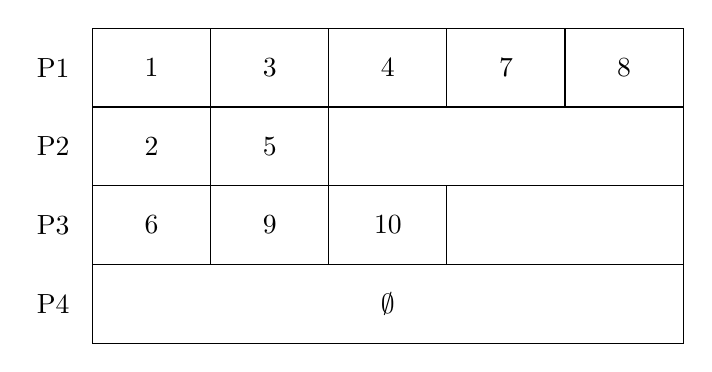
\begin{tikzpicture}
%\draw (0,0) rectangle (1.5,1);
\node at (-0.5,0.5) {P4};
\node at (-0.5,1.5) {P3};
\node at (-0.5,2.5) {P2};
\node at (-0.5,3.5) {P1};
\draw (0,1) rectangle (1.5,2) node[pos=.5] {$\tache{6}$};
\draw (0,2) rectangle (1.5,3) node[pos=.5] {$\tache{2}$};
\draw (0,3) rectangle (1.5,4) node[pos=.5] {$\tache{1}$};
\draw (1.5,1) rectangle (3,2) node[pos=.5] {$\tache{9}$};
\draw (1.5,2) rectangle (3,3) node[pos=.5] {$\tache{5}$};
\draw (1.5,3) rectangle (3,4) node[pos=.5] {$\tache{3}$};
\draw (3,1) rectangle (4.5,2) node[pos=.5] {$\tache{10}$};
\draw (3,3) rectangle (4.5,4) node[pos=.5] {$\tache{4}$};
\draw (4.5,3) rectangle (6,4) node[pos=.5] {$\tache{7}$};
\draw (6,3) rectangle (7.5,4) node[pos=.5] {$\tache{8}$};
\draw (0,0) rectangle (7.5,4);
\draw (0,0) rectangle (7.5,4);
\draw (0,0) rectangle (7.5,3);
\draw (0,0) rectangle (7.5,2);
\draw (0,0) rectangle (7.5,1) node[pos=.5] {$\emptyset$};
\end{tikzpicture}
\caption{Placement de taches en First Fit par les contraintes DM} \label{fig:exempleFF}
\end{center}
\end{figure}

\begin{figure}[!h]
\begin{center}
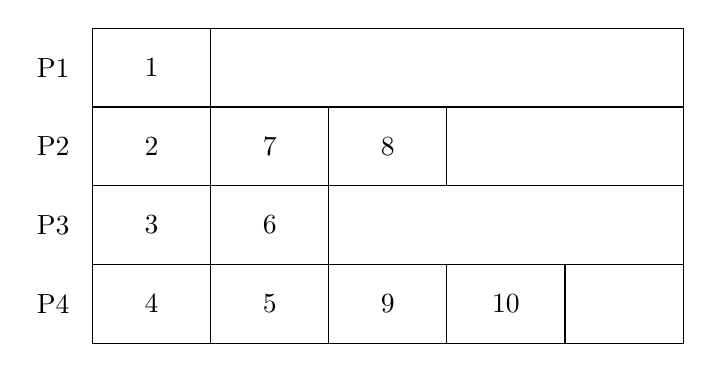
\begin{tikzpicture}
\node at (-0.5,0.5) {P4};
\node at (-0.5,1.5) {P3};
\node at (-0.5,2.5) {P2};
\node at (-0.5,3.5) {P1};
\draw (0,0) rectangle (1.5,1) node[pos=.5] {$\tache{4}$};
\draw (0,1) rectangle (1.5,2) node[pos=.5] {$\tache{3}$};
\draw (0,2) rectangle (1.5,3) node[pos=.5] {$\tache{2}$};
\draw (0,3) rectangle (1.5,4) node[pos=.5] {$\tache{1}$};

\draw (1.5,0) rectangle (3,1) node[pos=.5] {$\tache{5}$};
\draw (1.5,1) rectangle (3,2) node[pos=.5] {$\tache{6}$};
\draw (1.5,2) rectangle (3,3) node[pos=.5] {$\tache{7}$};

\draw (3,0) rectangle (4.5,1) node[pos=.5] {$\tache{9}$};
\draw (3,2) rectangle (4.5,3) node[pos=.5] {$\tache{8}$};

\draw (4.5,0) rectangle (6,1) node[pos=.5] {$\tache{10}$};
\draw (0,0) rectangle (7.5,4);
\draw (0,0) rectangle (7.5,4);
\draw (0,0) rectangle (7.5,3);
\draw (0,0) rectangle (7.5,2);
\draw (0,0) rectangle (7.5,1);
\end{tikzpicture}
\caption{Placement de taches en Best Fit par les contraintes DM} \label{fig:exempleBF}
\end{center}
\end{figure}

\vspace{1cm}
% \subsection{Algorithme d'ordonnancement utilisant une stratégie globale}
% \vspace{-1cm}
% Les algorithmes d'ordonnancement utilisant une stratégie globale n'entrant pas dans le cadre de ce mémoire, nous ne présenterons que succinctement les algorithmes les plus utilisés.
% \subsubsection{Algorithme de type Pfair}
% \vspace{-1cm}
% Les algorithmes de type Pfair ont la particularité d'exécuter les tâches à un taux régulier. Un algorithme Pfair a une caractéristique de limiter les variations du taux d’utilisation 
% en s'assurant que le taux d'exécution de la tâche $\periode{i}$ reste voisin de $U_i$, quelle que soit la longueur de l'intervalle considéré.

% Parmi les algorithmes d'ordonnancement Pfair, nous pouvons citer :
% \begin{itemize}
% \item[$\bullet$] PF \cite{BCPV96}
% \item[$\bullet$] PD \cite{BGP95}
% \item[$\bullet$] PD2 \cite{AS00}
% \end{itemize}

\section{Conclusion}
\vspace{-1cm}
\chapter{Etat de l'art}
\minitoc
\section{Introduction}
\section{Les modèles de consommation d'énergie DVFS et DPM}
\vspace{-1cm}
L’énergie consommée par un processeur est l'integrale de la puissance dissipée et du temps d’exécution. Nous utiliserons principalement la notion de consommation énergétique et non de puissance. Cette consommation énergétique est divisée en consommation statique et consommation dynamique. Nous détaillons dans cette section les modèles des consommations dynamique et statique et montrons que la consommation statique est récemment devenue plus importante que la consommation dynamique.
\subsection{Consommation dynamique}
\vspace{-1cm}
% La fréquence et la tension d’alimentation des processeurs sont liées. Lorsqu’un processeur possède plusieurs fréquences de fonctionnement, chaque fréquence peut fonctionner avec au maximum seulement une ou deux tensions d’alimentation et la consommation énergétique du processeur dépend à la fois de la fréquence et de la tension d’alimentation utilisées.
% \\ \indent La puissance dynamique est dissipée lors de la commutation des composants et dépend donc de la fréquence f du processeur. Elle peut être approximée selon la relation suivante \cite{CK07} : 
Mei et al.\cite{Mei13}, ont défini la dissipation de puissance dynamique par un circuit CMOS comme produit de
Un coefficient constant qui dépend de la technologie utilisée pour fabriquer la puce, par la
Carré de la tension et par la fréquence.
\begin{equation}
\pow_{dynamique} = \coeff * \freq * \volt^2 
\end{equation}
Où $\coeff$ correspond à la capacité de sortie du circuit et $\volt$ à la tension d’alimentation. 	
\\ \indent Les solutions permettant de réduire la puissance dynamique dans les circuits s’attachent par conséquent à réduire la fréquence de fonctionnement. La relation précédente montre qu’il est moins économique d’un point de vue énergétique de faire fonctionner un circuit à pleine vitesse que de faire fonctionner un circuit à vitesse réduite pendant un laps de temps plus important.
\\ \indent La technique permettant de réduire la vitesse du système est appelée DVFS (Dynamic Voltage and Frequency Scaling) et tire parti du fait que les processeurs ont plusieurs fréquences et plusieurs tensions de fonctionnement. De nombreux algorithmes d’ordonnancement ont été proposés utilisant cette solution \cite{WWDS94, YDS95, PS01}.
\subsection{Consommation statique}
\vspace{-1cm}
La consommation statique des processeurs est en grande partie due aux courants de fuite. 
Dans un circuit idéal, cette consommation statique est nulle mais, en réalité, un courant 
de fuite existe et est responsable d’une consommation énergétique non négligeable. 
Ce courant de fuite provient du fait que les transistors composant le circuit ne sont pas parfaits. 
La consommation statique peut être modélisée comme une constante \cite{KAB+03, SJPL08}.
Plusieurs solutions matérielles existent pour réduire la consommation statique. 
L’idée générale est d’éteindre une partie du circuit qui n’est pas utilisée pour qu’aucun courant de fuite ne circule. 
Cette solution est appelée Power Gating. Dans les circuits actuels, les puces peuvent être divisées en plusieurs parties, 
chaque partie ayant la possibilité d’être éteinte indépendamment des autres parties du circuit. Certaines sources \cite{HXW+10} 
affirme que l’énergie statique représente jusqu’à 70\% de la consommation énergétique totale dissipée par un processeur. 
Plusieurs études confirment cette affirmation \cite{Bor99, SBA+01, KAB+03, ABM+04, HSC+11, BBMB13}. Des expériences ont également été faites 
\cite{SRH05, SPH05, LSH10} en utilisant les algorithmes d’ordonnancement existants et les conclusions de ces études est que réduire uniquement 
la consommation dynamique peut entraîner une hausse de la consommation énergétique globale car les composants sont actifs plus longtemps ce 
qui entraîne une hausse de la consommation statique.

\section{Les états C-states du processeur}
\vspace{-1cm}
\label{sec:cstate}
Pour réduire la consommation statique des processeurs, 
il est nécessaire d’utiliser leurs états basse-consommation lors de leurs périodes d’inactivité. 
Nous appelons périodes d’inactivité les périodes de temps durant lesquelles un processeur est inactif et où aucune tâche n’est exécutée. 
Les processeurs disposent maintenant de plusieurs états basse-consommation où un certain nombre de composants sont désactivés pour réduire la consommation énergétique. 
Le problème lié à l’utilisation de ces états basse-consommation est qu’éteindre, rallumer ou changer d’état un processeur n’est pas anodin, que ce soit du point de vue 
énergétique ou temporel. Nous définissons dans cette section quatre notions relatives aux états basse-consommation. Nous notons ns le nombre d’états basse-consommation 
de chaque processeur et nous supposons que tous les processeurs possèdent les mêmes états basse-consommation.

Consommation énergétique. Nous notons $Cons_s$ la consommation énergétique de l’état basse-consommation s. C’est la consommation énergétique dépensée lorsque le processeur 
se trouve dans cet état basse-consommation. 
Elle dépend du nombre de composants qui ont été désactivés. 
Plus ce nombre est important, plus la consommation énergétique sera réduite.

Délai de transition. Nous définissons le délai de transition d’un état basse-consommation comme le temps nécessaire pour revenir de cet état basse-consommation à l’état actif.
 C’est le temps nécessaire pour réactiver tous les composants éteints durant l’état basse-consommation. 
 Le délai de transition de l’état basse-consommation s est noté $Del_s$. 
 Plus la consommation énergétique de l’état basse-consommation est faible, 
 plus son délai de transition va être important car davantage de composants devront été réactivés.

Pénalité énergétique. Nous notons $Pen_s$ la pénalité énergétique pour revenir de l’état basse-consommation s à l’état actif.
Cette pénalité énergétique correspond à la consommation énergétique nécessaire pour réactiver tous les composants qui ont été 
éteints lors de l’activation de l’état basse-consommation. Elle est consommée lorsque le processeur passe de l’état basse-consommation à l’état actif, 
c’est-à-dire lors du délai de transition. Plus la consommation énergétique d’un état basse-consommation est faible, plus sa pénalité est importante.
nous faisons l’hypothèse que l’évolution de la consommation énergétique lors du réveil du processeur est linéaire. En supposant que la consommation énergétique à l’état actif est de $Cons_{actif}$,
la pénalité énergétique d’un état basse-consommation est donc donnée par la formule suivante :
\begin{equation}
Pen_s = \frac{1}{2} \times Del_s \times (Cons_{actif} - Cons_s)
\end{equation}
Nous faisons cette hypothèse car les pénalités énergétiques des états basse-consommation sont difficiles à obtenir, 
les constructeurs ne fournissant généralement que les valeurs des délais de transition pour revenir des différents états basse-consommation 
(e.g. \cite{STM, MPC}). Néanmoins, nos contributions ne dépendent pas de cette modélisation qui n’est utilisée que pour les évaluations et qui 
peut être modifiée si les pénalités énergétiques des états basse-consommation sont connues.

Break Even Time (BET). Nous définissons le BET comme la largeur minimale de la pé-riode d’inactivité pour qu’il soit possible d’activer un état basse-consommation \cite{AP11, CG06, DA08a}.
 Chaque état basse-consommation possède donc son propre BET et nous nommons $BET$ le BET de l’état basse-consommation s. 
 Le BET de l’état basse-consommation s correspond à la période de temps pour laquelle la consommation énergétique du processeur à l’état actif est égale à la consommation énergétique
 dans l’état basse-consommation s (i.e. $Cons_s$) plus sa pénalité énergétique (i.e. $Pen_s$). Si la longueur d’une période d’inactivité est inférieure au BET d’un état basse-consommation
 donné, il est alors plus efficace énergétiquement de laisser le processeur dans son état actif que d’activer l’état basse-consommation en question. À noter que le BET ne permet pas de savoir 
 si une contrainte temps réel va être violée si cet état basse-consommation est activé. C’est le délai de transition de l’état basse-consommation qui importe alors pour réveiller à temps le processeur.

Comme vu ci-dessus, nous faisons l’hypothèse que la consommation énergétique évolue linéairement pour revenir de la consommation énergétique d’un état basse-consommation à celle de l’état actif. 
Avec cette hypothèse, le BET et le délai de transition d’un état basse-consommation sont égaux. 
En d’autre termes, il est toujours plus efficace d’activer un état basse-consommation que de laisser le processeur dans l’état actif si la longueur de la période d’inactivité 
est supérieure au délai de transition d’un état basse-consommation. De même que pour la pénalité énergétique, nous n’utilisons cette hypothèse que dans nos évaluations et 
nos contributions séparent les notions de BET et de délai de transition.
Exemples de processeurs

La majorité des processeurs actuels disposent de plusieurs fréquences de fonctionnement et d’états basse-consommation pour réduire leur consommation énergétique, nous en détaillons quelques-uns ici. Comme notre objectif est de réduire la consommation statique, nous ne détaillons pas les fréquences disponibles. Nous détaillons en revanche les caractéristiques de chaque état basse-consommation, i.e. quels sont les composants éteints et quelles sont les étapes requises pour retrouver l’état actif.

Parmi les processeurs utilisés dans la littérature, citons le Freescale MPC8536 \cite{MPC} utilisé par Awan et al. \cite{AP11, AP13, AYP13}. Ce processeur est basé sur une architecture PowerPC. Ses états basse-consommation sont détaillés dans le Tableau 2.4.
\section{L'endormissement de processeur (Online VS Offline)}
\vspace{-1cm}
\section{Le Modèle d'endormissement de Dsouza}
\vspace{-1cm}
Anthony Rowe a proposé un algorithme d’ordonnancement appellé "Energy Saving Rate Harmonized Scheduling (ES RHS)" \cite{Rowe10} basé sur la période d’harmonisation qui améliore la consommation d’énergie pour l’architecture multiprocesseur.
Dsouza l'a amelioré en proposant "ES RHS+" dans cette section nous définirons la periode harmonique, puis nous presenterons l'algorithme "Rate Harmonized Scheduling" et "Energy Saving Rate-Harmonized Scheduling" enfin nous terminerons par l'algorithme "Energy-Saving Rate-Harmonized Scheduling".

\subsection{Période d’harmonisation}

Soit un ensemble $\taskset$ de tache de n taches périodiques indépendantes, l’ensemble de tâche est ordonnée selon les périodes de chaque tache de tel façon que $\periode{1} \leq \periode{2} \leq \dots \leq \periode{n}$. 
Un ensemble de taches $\{\tache{1}, \tache{2}, \dots, \tache{n} \}$ est harmonique si il existe un $\periode{H}$ tel que $\forall \tache{i} / \frac{\periode{i}}{\periode{H}} \in \mathbb{Z}$

\subsection{Algorithme d’ordonnancement « Energy-Saving Rate-Harmonized Scheduling »}

En général RHS utilise un ensemble de Valeurs périodiques \{ $\periode{H}^1,\periode{H}^2,\dots ,\periode{H}^3$ \} où $\periode{H}^i \leq \periode{i}$ pour i = 1 .. n, Et les valeurs sont harmoniques. Les périodes harmoniques sont appelées "périodes de base harmonisées", Et toute les taches ont le même temps de reveil de $\tache{1}$ = $\rev1$ = 0.
\\ Les tâches $\{\tache{1}, \tache{2}, \dots, \tache{n} \}$ dans l’ensemble tâches donné sont réveillées selon leurs arrivée comme dans le modèle classique Toutefois, chaque job de $\tache{i}$ ne peut être exécutée que à sa prochaine frontière périodique la plus proche de $\periode{H}^i$ \cite{Rowe10}.
\\ \indent Dans le L’ordonnancement RHS de base, \{ $\periode{H}^1 = \periode{H}^2 = … = \periode{H}^n = \periode{H}$ \}, $\periode{H}$ Est simplement appelé période d'harmonisation et $\periode{H} \leq \periode{1}$. Les tâches qui arrivent avant ou après les multiples entiers de $\periode{H}$ ne sont pas autorisée à s'exécuter jusqu'à la prochaine limite la plus proche de quand ils sont lancés en fonction de leur priorité (voir figure). Les tâches qui ne sont pas admissibles sont retardées jusqu'à la prochaine limite.
\\ \indent $\periode{H}$ est choisi de manière à améliorer l'ordonnancement \cite{Rowe10}. Supposer $\Psi~=~\{ \tache{j} / \periode{j}~<~2\periode{1},~j~\neq 1\}$. si $\Psi = \emptyset, \periode{H} = \periode{1}.~sinon~\periode{H} = \frac{\periode{1}}{2}$. 

\begin{theoreme}[\cite{Rowe10}]
un ensmeble de taches $\taskset$ est faisable sous RHS si $U \leq 0.5$ .
\end{theoreme}

\begin{theoreme}
le calcul du pire temps de reponse $W_k$ [23,24] dans le cas de RHS peut etre redéfini comme suit :
\\ 
%\begin{equation}
\begin{align}
W_0 & = \wcet{i} + \periode{H} 
\\ W_{k+1} & = \wcet{i} + \periode{H} + \sum_{j = 1}^{i-1} \bigg \lceil \frac{W_k}{\periode{j}}\bigg \rceil \wcet{j}
\end{align}
%\end{equation}
\end{theoreme}

\begin{theoreme}[\cite{Rowe10}]
Soit $\taskset = \{\tache{1}, \tache{2}, \dots, \tache{n} \}$ un ensemble de tache periodiques indépendantes. \\
Si il existe une tache $\tache{i}$ avec un pire temps de reponse $W_k$ tel que $W_k > \deadline{i}$ alors l'ensemble de tache $\taskset$ est non ordonnançable.
\end{theoreme}
\subsection{Energy-Saving Rate-Harmonized Scheduling}
comme vu dans la section \ref{sec:cstate}, les processeurs sont dotés de mode de basse consommation.
par exemple: un processeur "power-aware" a :
\vspace{0.5cm}
\begin{itemize}
\item[$\bullet$] mode actif avec une consommation d'énergie $PW_{active}$
\item[$\bullet$] mode sommeil avec une consommation d'énergie $PW_{idle}$ et un temps de bascule $ST_{idle}$
\item[$\bullet$] mode sommeil profond avec une consommation d'énergie $PW_{sleep}$ et un temps de bascule $ST_{sleep}$
\end{itemize}
\vspace{0.5cm}
avec $PW_{active} > PW_{idle} \gg PW_{sleep} $ et $ ST_{idle} \ll ST_{sleep}$.
\\ \indent quand il n'y a aucune tache préte à s'executer, le processeur et generalement en mode sommeil, cependant si il  y a une tache qui arrive avant $\S\periode{sleep}$ unité de temps,il ne peut passer en mode sommeil.
\\ \indent ES-RHS présente une propriété intéressante, où tous les periode de sommeil précède et est contiguë au sommeil profond durée peuvent toujours être fusionnée [10]. Par conséquent, en harmonisant
les exécutions de tâches non harmoniques, ES-RHS peut produire des periode de sommeil optimal. D'souza \cite{DAR16} a redéfini la notion d'harmonisation pour ameliorer l'ordonnancemen ES-RHS.
\subsection{Energy-Saving Rate-Harmonized Scheduling+}
\indent Une tâche est susceptible d'être exécutée lorsque le processeur est occupé ou une limite de la période d'harmonisation a été atteinte. Cette redéfinition permet aux taches d'etre préte à s'executer plus tôt par rapport à l'ordonnanceur de ES-RHS \cite{Rowe10}.
\\ la table \ref{tab:exempleRHS} et les figures \ref{fig:exempleRHS} et \ref{fig:exempleRHS+} illustrent la difference entre les deux ordonnanceur et l'apport de D'souza.

\begin{table}[h]
\begin{center}
\begin{tabular}{|c|c|c|}
 \hline$\tache{i}$ & $\wcet{i}$ & $\periode{i}$ \\ 
 \hline1 & 1 & 10 \\ 
 \hline 2 & 4 & 23 \\ 
 \hline 3 & 3 & 36 \\ 
 \hline 
 \end{tabular}
\end{center}
\caption{Ensemble de taches} \label{tab:exempleRHS}
\end{table}

\begin{center}
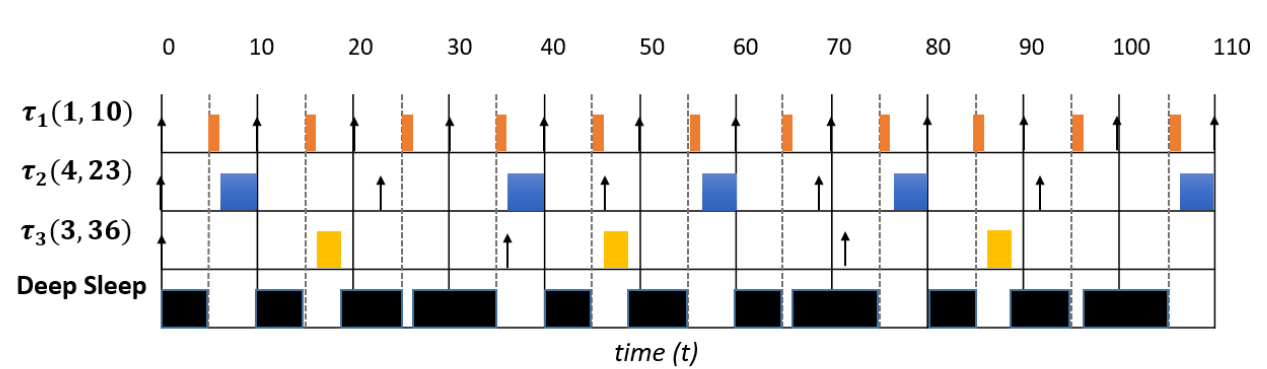
\includegraphics[height=4cm,width=12cm]{rhs.png}
\captionof{figure}{Energy-Saving RHS}
\label{fig:exempleRHS}
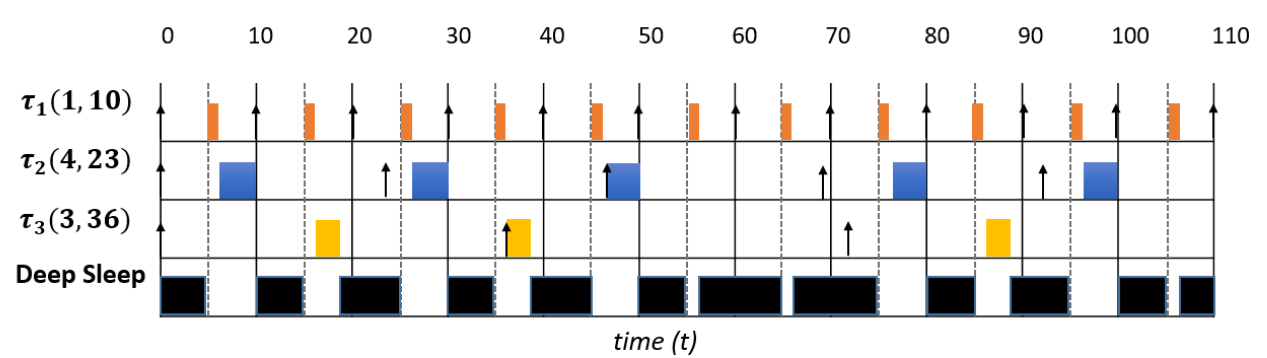
\includegraphics[height=4cm,width=12cm]{rhs+.png}
\captionof{figure}{Energy-Saving RHS+}
\label{fig:exempleRHS+}
\end{center}

\section{Conclusion}
\vspace{-1cm}